\section{Results}
\label{sec:results}

Table~\ref{tab:generalization-results} separates endpoint generalization from layout and dynamics shifts. The full RL policy changes from 96.0\% success on the training layout with held-out endpoints to 90.0\% on unseen matched-density layouts and 72.0\% on denser layouts. The three classical planners remain at 100\% on these splits, so the experiment provides no reliability advantage for the learned method. Scaling exposes the strongest boundary: RL success is 98.0\%, 56.0\%, 14.0\%, and 0.0\% at grid widths 15, 30, 50, and 100, while every classical planner remains at 100\%. At $100\times100$, the full RL policy uses 932.266 ms of route decision time versus 3.566 ms for A*. Thus, these implementations show no scale crossover in favor of RL.

The held-out-pair ablation in Table~\ref{tab:ablation-results} is also non-monotonic. Vanilla DQN and the full-grid observation reach only 38.0\% and 15.3\%, respectively, supporting Double DQN and the local observation in this setup. Yet removing HER (100.0\%), shaping (100.0\%), or the curriculum (100.0\%) each exceeds the full method's 96.0\% on this split. These one-factor interventions show configuration sensitivity, not separable causal main effects, because the learning components interact.

At matched change events, the full RL method attains 87.9\% post-change success, while its recovery criterion is met in 100.0\% of observed events. This distinction matters: recovery of optimal remaining cost before termination does not guarantee that the complete route succeeds. The corresponding D* Lite values are 100.0\% and 100.0\%.


\subsection{Generalization}
\begin{table}[H]
\centering
\caption{Generalization summary (mean $\pm$ 95\% CI). C succ. is the minimum success among A*, Dijkstra, and D* Lite; RL estimates use five policies and gap uses successful routes.}
\scriptsize
\setlength{\tabcolsep}{2.4pt}
\resizebox{\columnwidth}{!}{%
\begin{tabular}{lrrrrr}
\toprule
Condition & C succ. (\%) & RL succ. (\%) & RL gap & A* ms & RL ms \\
\midrule
Held-out pairs & 100.0 & $96.0 \pm 11.1$ & $1.11 \pm 0.45$ & $0.15 \pm 0.02$ & $6.61 \pm 9.77$ \\
Unseen layout & 100.0 & $90.0 \pm 5.9$ & $0.90 \pm 0.38$ & $0.16 \pm 0.04$ & $11.16 \pm 3.79$ \\
Denser layout & 100.0 & $72.0 \pm 8.6$ & $0.92 \pm 0.38$ & $0.18 \pm 0.04$ & $26.32 \pm 6.95$ \\
New obstacle sites & 100.0 & $98.0 \pm 5.6$ & $0.93 \pm 0.17$ & $0.20 \pm 0.05$ & $4.59 \pm 2.86$ \\
New toggle periods & 100.0 & $98.7 \pm 3.7$ & $0.88 \pm 0.35$ & $0.48 \pm 0.14$ & $4.86 \pm 3.28$ \\
\bottomrule
\end{tabular}%
}
\label{tab:generalization-results}
\end{table}


\IfFileExists{figures/generalization_success.pdf}{
\begin{figure*}[t]
    \centering
    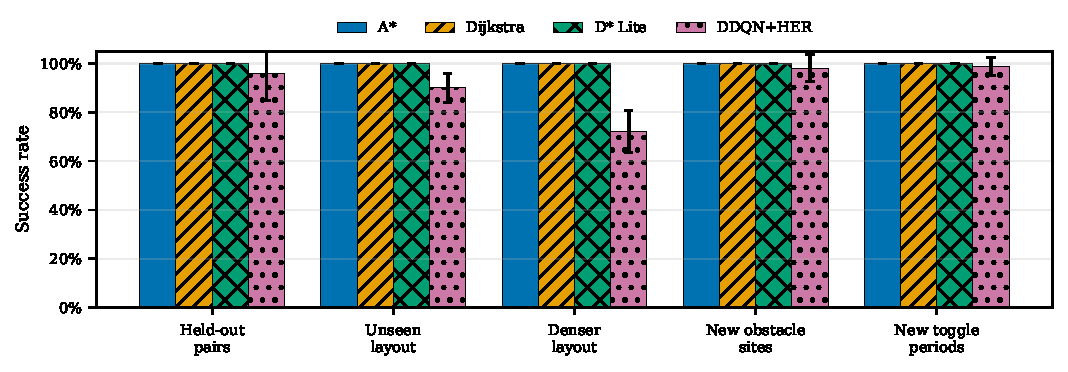
\includegraphics[width=0.96\textwidth]{figures/generalization_success.pdf}
    \caption{Generalization under paired benchmark conditions. Classical bars
    aggregate scenarios; DDQN+HER error bars are 95\% confidence intervals
    across five independently trained policies. Hatches preserve distinctions
    in grayscale.}
    \label{fig:generalization-success}
\end{figure*}
}{}

\subsection{Scaling}
\begin{table}[H]
\centering
\caption{Scaling summary (mean $\pm$ 95\% CI). C succ. is the minimum success among A*, Dijkstra, and D* Lite; RL estimates use five policies and gap uses successful routes.}
\scriptsize
\setlength{\tabcolsep}{2.4pt}
\resizebox{\columnwidth}{!}{%
\begin{tabular}{lrrrrr}
\toprule
Condition & C succ. (\%) & RL succ. (\%) & RL gap & A* ms & RL ms \\
\midrule
$15\times15$ & 100.0 & $98.0 \pm 5.6$ & $1.57 \pm 0.48$ & $0.32 \pm 0.12$ & $4.39 \pm 1.09$ \\
$30\times30$ & 100.0 & $56.0 \pm 28.6$ & $2.89 \pm 2.21$ & $0.51 \pm 0.21$ & $115.57 \pm 94.04$ \\
$50\times50$ & 100.0 & $14.0 \pm 16.7$ & $4.10 \pm 9.01$ & $0.98 \pm 0.61$ & $485.83 \pm 221.62$ \\
$100\times100$ & 100.0 & $0.0 \pm 0.0$ & -- & $3.57 \pm 2.05$ & $932.27 \pm 1103.25$ \\
\bottomrule
\end{tabular}%
}
\label{tab:scaling-results}
\end{table}


\IfFileExists{figures/scaling_overview.pdf}{
\begin{figure*}[t]
    \centering
    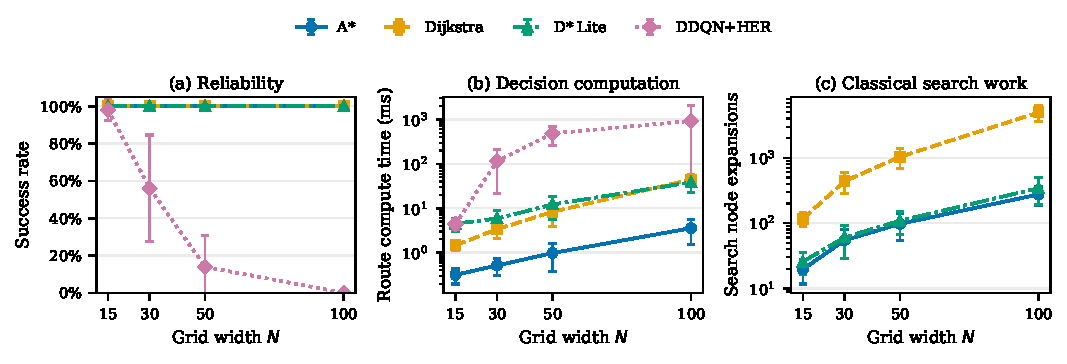
\includegraphics[width=0.98\textwidth]{figures/scaling_overview.pdf}
    \caption{Scaling behavior: (a) reliability, (b) route-level decision
    computation on a logarithmic axis, and (c) classical search work on a
    logarithmic axis. Model-free RL has no search-node expansion count.}
    \label{fig:scaling-overview}
\end{figure*}
}{}

\subsection{Controlled Realism Factors}
\begin{table}[H]
\centering
\caption{Controlled realism summary (mean $\pm$ 95\% CI). C succ. is the minimum success among the three classical planners; RL gap uses successful routes.}
\scriptsize
\setlength{\tabcolsep}{2.4pt}
\resizebox{\columnwidth}{!}{%
\begin{tabular}{lrrrrr}
\toprule
Condition & C succ. (\%) & RL succ. (\%) & RL gap & A* ms & RL ms \\
\midrule
Static density 0.40 & 100.0 & $72.0 \pm 26.9$ & $1.32 \pm 0.45$ & $0.19 \pm 0.05$ & $26.29 \pm 20.59$ \\
Stochastic toggle 0.20 & 100.0 & $100.0 \pm 0.0$ & $1.18 \pm 0.45$ & $0.39 \pm 0.15$ & $4.11 \pm 0.69$ \\
Moving obstacle, $T=2$ & 100.0 & $100.0 \pm 0.0$ & $1.32 \pm 0.33$ & $0.66 \pm 0.23$ & $5.82 \pm 0.93$ \\
Energy penalty 1.0 & 100.0 & $100.0 \pm 0.0$ & $1.98 \pm 0.54$ & $0.15 \pm 0.04$ & $2.93 \pm 0.27$ \\
Hard no-fly & 100.0 & $78.0 \pm 26.9$ & $1.58 \pm 0.40$ & $0.17 \pm 0.08$ & $16.55 \pm 14.76$ \\
Penalized no-fly & 100.0 & $92.0 \pm 16.2$ & $1.75 \pm 0.53$ & $0.33 \pm 0.14$ & $10.79 \pm 14.32$ \\
Sensor noise 0.10 & 100.0 & $100.0 \pm 0.0$ & $1.44 \pm 0.37$ & $0.31 \pm 0.11$ & $3.77 \pm 0.64$ \\
\bottomrule
\end{tabular}%
}
\label{tab:realism-results}
\end{table}


\subsection{RL Ablations}
\begin{table}[H]
\centering
\caption{Held-out-pair ablations across five policy seeds (mean $\pm$ 95\% CI); an interval is omitted when fewer than two finite seed estimates are available.}
\scriptsize
\setlength{\tabcolsep}{2.7pt}
\begin{tabular}{lrrr}
\toprule
Variant & Success (\%) & Cost gap & Route ms \\
\midrule
DQN+HER & $38.0 \pm 63.0$ & $0.63 \pm 1.39$ & $53.00 \pm 55.69$ \\
Dynamic-only train & $92.0 \pm 20.0$ & $1.13 \pm 0.43$ & $8.20 \pm 11.63$ \\
DDQN+HER & $96.0 \pm 11.1$ & $1.11 \pm 0.45$ & $6.61 \pm 9.77$ \\
Full-grid obs. & $15.3 \pm 42.6$ & 3.18 & $13.84 \pm 5.93$ \\
No curriculum & $100.0 \pm 0.0$ & $0.87 \pm 0.16$ & $3.55 \pm 0.71$ \\
No HER & $100.0 \pm 0.0$ & $1.01 \pm 0.14$ & $3.47 \pm 0.69$ \\
No shaping & $100.0 \pm 0.0$ & $0.92 \pm 0.41$ & $3.21 \pm 0.50$ \\
\bottomrule
\end{tabular}
\label{tab:ablation-results}
\end{table}


\subsection{Event-Level Adaptability}

\begin{table}[H]
\centering
\caption{Event-level adaptability across all dynamic scenarios. Values are means and 95\% confidence intervals over independent scenarios for classical planners and policy seeds for RL.}
\scriptsize
\setlength{\tabcolsep}{2.3pt}
\resizebox{\columnwidth}{!}{%
\begin{tabular}{lrrrrr}
\toprule
Method & $n$ & Post-success (\%) & Recovery (\%) & Cost shock & Reaction ms \\
\midrule
A* & 83 & $100.0 \pm 0.0$ & $100.0 \pm 0.0$ & $0.000 \pm 0.000$ & $0.067 \pm 0.007$ \\
Dijkstra & 83 & $100.0 \pm 0.0$ & $100.0 \pm 0.0$ & $0.001 \pm 0.002$ & $0.442 \pm 0.062$ \\
D* Lite & 83 & $100.0 \pm 0.0$ & $100.0 \pm 0.0$ & $0.005 \pm 0.008$ & $0.168 \pm 0.018$ \\
DDQN+HER & 5 & $87.9 \pm 33.6$ & $100.0 \pm 0.0$ & $0.005 \pm 0.002$ & $0.521 \pm 0.050$ \\
\bottomrule
\end{tabular}%
}
\label{tab:adaptability-results}
\end{table}


The dedicated event files report optimal-cost shock, positive extra optimal
cost attributable to the change, recovery steps, post-change success, reaction
time, and search expansions for every change.
Events that do not recover before termination remain in the denominator and
retain a missing recovery time. This avoids the optimistic bias that would
result from analyzing only recovered or successful events.

\IfFileExists{figures/adaptability_recovery.pdf}{
\begin{figure}[t]
    \centering
    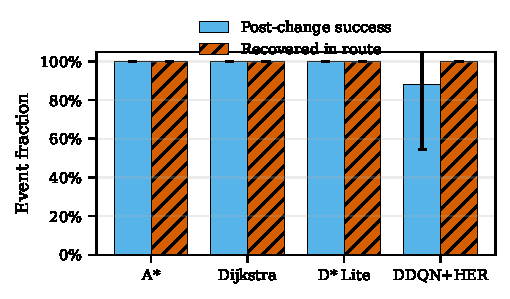
\includegraphics[width=\linewidth]{figures/adaptability_recovery.pdf}
    \caption{Post-change route success and recovery before termination across
    all dynamic scenarios.}
    \label{fig:adaptability-recovery}
\end{figure}
}{}

\IfFileExists{figures/adaptability_reaction_time.pdf}{
\begin{figure}[t]
    \centering
    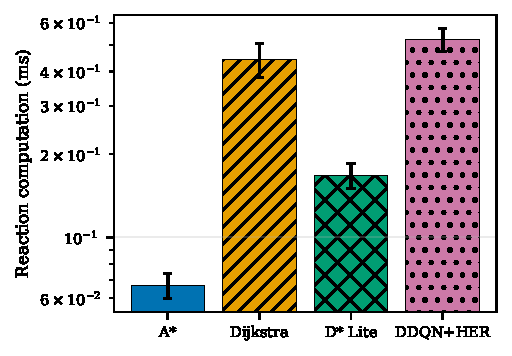
\includegraphics[width=\linewidth]{figures/adaptability_reaction_time.pdf}
    \caption{Event reaction computation on a logarithmic scale. Classical
    values time the repair; RL values time the first post-change decision.}
    \label{fig:adaptability-reaction}
\end{figure}
}{}

\subsection{Paired Statistical Tests}

The machine-readable paired-test artifact reports exact McNemar tests for
success and Wilcoxon signed-rank tests for cost and compute time, together with
rank-biserial effect sizes and Holm-adjusted $p$-values. Seed-specific RL
comparisons remain separate in the raw statistical output; aggregate confidence
intervals are computed from seed-level estimates rather than treating routes
from one policy as independent trained agents. A second paired-test artifact
applies the same controls to matched change events, using change step and
changed-cell signature rather than event order alone.
The exhaustive family contains 13,014 route-level tests and is deliberately
conservative. As one concrete effect, A* is faster than DDQN+HER on every
denser-layout seed comparison (Wilcoxon rank-biserial effect $=1.0$;
globally Holm-adjusted $p=2.24\times10^{-5}$ for each seed). Success and cost
effects should be read with their confidence intervals and adjusted tests,
not with uncorrected route-level significance.
